\documentclass[t,aspectratio=169]{beamer}
\usepackage[utf8]{inputenc}
\usepackage[T1]{fontenc}
\usepackage{xcolor}
\usepackage{hyperref}
\usepackage{tikz}
\usepackage{pgfplots}
\pgfplotsset{compat=1.8}
\usepackage{adjustbox}
\usepackage{tabularx}
\usepackage{array}
\usepackage{fontspec}
\usefonttheme{serif} % default family is serif

\title{Bayesian data analysis with TensorFlow Probability}
\date{DataScienceConference Europe 2020}
\author{Simeon Carstens \& Dorran Howell, Tweag I/O}
\newcommand{\todo}{\textcolor{red}{\textbf{TODO}}}
\renewcommand{\d}{\mathrm{d}}
\setmainfont{Roboto}
\usetheme{tweag}

\begin{document}

\begin{frame}
  \titlepage
\end{frame}


\begin{frame}
  \frametitle{Your hosts}
  \begin{tcolorbox}[title=Simeon will give the presentation]
    \begin{minipage}{0.3\textwidth}{
        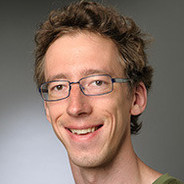
\includegraphics[width=0.15\paperwidth]{images/simeon}}
    \end{minipage}
    \begin{minipage}{0.6\textwidth}
    \begin{itemize}
    \item background in computational biology
    \item Data Scientist at Tweag since 2019
    \end{itemize}
    \end{minipage}
  \end{tcolorbox}

  \begin{tcolorbox}[title=Dorran will happily answer questions]
    \begin{minipage}{0.3\textwidth}{
        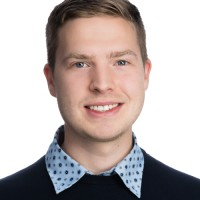
\includegraphics[width=0.15\paperwidth]{images/dorran}}
    \end{minipage}
    \begin{minipage}{0.6\textwidth}
    \begin{itemize}
    \item previous positions in geophysics
    \item Data Scientist at Tweag since 2019
    \end{itemize}
    \end{minipage}
  \end{tcolorbox}
\end{frame}


\begin{frame}
  \frametitle{Tweag I/O}
  \todo \\
  Tweag I/O is a software innovation lab and consultancy based in Paris with employees all around the world.\\
  We specialize in
  \begin{itemize}
  \item software engineering, with a focus on functional programming
  \item DevOps, with a focus on reproducible software systems and builds
  \item data science
  \end{itemize}
\end{frame}


\begin{frame}
  \frametitle{What you're in for}
  This tutorial consists of alternating blocks of
  \begin{itemize}
  \item theory / example slides
  \item practical examples on either external websites or Google Colab notebooks. Links are provided at {\centering \url{https://github.com/tweag/tutorial-dsc-2020/}}
  \end{itemize}

  Requirements:
  \begin{itemize}
  \item a Google account (for the practical exercises)
  \item elementary knowledge in probability theory and statistics
  \end{itemize}
\end{frame}

\pgfmathdeclarefunction{gauss}{2}{%
  \pgfmathparse{1/(#2*sqrt(2*pi))*exp(-((x-#1)^2)/(2*#2^2))}%
}

\tikzset{
  normal/.pic={
    \begin{tikzpicture}
      \begin{axis}[
        axis lines = left,
        xlabel = $x$,
        ylabel = {$p(x)$},
        width=0.4\textwidth
        ]
        \addplot [
        domain=-4:4, 
        samples=200, 
        color=black,
        ]
        {gauss(0,1)};
      \end{axis}
    \end{tikzpicture}
  }
}


\tikzset{
  coin_prior/.pic={
    \begin{tikzpicture}
      \begin{axis}[
        axis lines = left,
        xlabel = $b$,
        ylabel = {$p(b)$}
        width=0.5\textwidth
        ]
        \addplot [
        domain=0:1, 
        samples=100, 
        color=black,
        ]
        {x^0.5 * (1 - x)^0.5};
      \end{axis}
    \end{tikzpicture}
  }
}

\tikzset{
  coin_likelihood/.pic={
    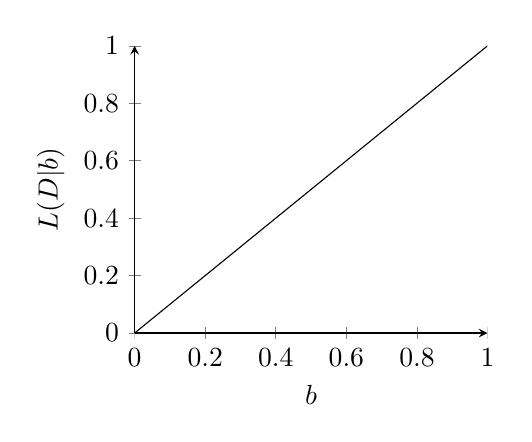
\begin{tikzpicture}
      \begin{axis}[
        axis lines = left,
        xlabel = $b$,
        ylabel = {$L(D|b)$},
        width=0.5\textwidth
        ]
        \addplot [
        domain=0:1, 
        samples=100, 
        color=black,
        ]
        {x};
      \end{axis}
    \end{tikzpicture} 
  }
}


\tikzset{
  coin_posterior/.pic={
    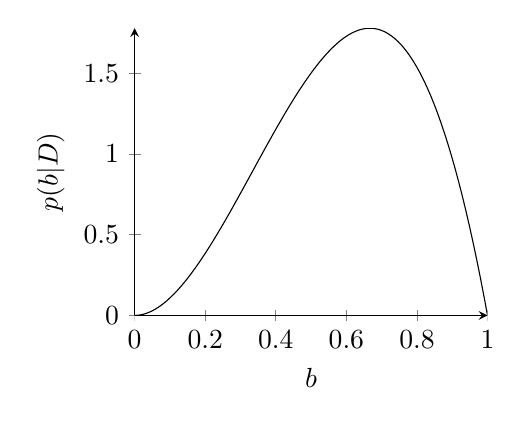
\begin{tikzpicture}
      \begin{axis}[
        axis lines = left,
        xlabel = $b$,
        ylabel = {$p(b|D)$},
        width=.5\textwidth
        ]
        \addplot [
        domain=0:1, 
        samples=100, 
        color=black,
        ]
        {x^2 * (1 - x) * 12};
      \end{axis}
    \end{tikzpicture}
  }
}

\begin{frame}
  \frametitle{Reminder: Probabilities}
  Probability distributions can be...
  \begin{tabular}{ m{2cm} m{7cm} m{5cm}}
    discrete: & $\mathrm{Ber(k; b)}=b^k(1-b)^{1-k}$ & \raisebox{-0.5\height}{\adjustbox{width=0.15\textwidth}{\tikz \pic{normal};}} \\
    continuous: & $\mathrm{\mathcal{N}(x; \mu, \sigma)}=\frac{1}{\sqrt{2 \pi \sigma^2}}\exp(-\frac{1}{2\sigma^2}(x-\mu)^2)$ & \raisebox{-0.5\height}{\adjustbox{width=0.15\textwidth}{\tikz \pic{normal};}}
  \end{tabular}\\
  Important concepts:
  \begin{description}
  \item[Conditional probability] \hfill \\ $p(A|B)$: probability that $A$ is true, given $B$ is true
  \item[Joint probability] \hfill \\  $p(A,B)$: probability that both $A$ and $B$ are true
  \item[Conditional joint probability] \hfill \\  $p(A,B|C)$: probability that both $A$ and $B$ are true, given $C$ is true
  \end{description}
\end{frame}


\begin{frame}
  \frametitle{Bayesian vs frequentist probabilities}
  Example: fair coin flip with $p(\mathrm{head}) = p(\mathrm{tail}) = \frac{1}{2}$
  \begin{tcolorbox}{Frequentist probability}
    \begin{description}
    \item[$p(\mathrm{"flip\ results\ in\ head"}|b=\frac{1}{2})=\frac{1}{2}$:] \hfill \\ $\frac{\mathrm{\# \ of \ heads}}{\mathrm{\# \ total \ flips}}$ for $\infty$ many fair coin flips
    \end{description}
  \end{tcolorbox}
  \begin{tcolorbox}{Bayesian probability}
    \begin{description}
    \item[$p(\mathrm{"flip\ results\ in\ head"}|b=\frac{1}{2})=\frac{1}{2}$:] \hfill \\ measure of \textit{belief} in the statement ``flip results in head'' given single fair coin flip
    \end{description}
  \end{tcolorbox}
  \todo: this slide looks complicated and is aesthetically offputting
\end{frame}


\begin{frame}
  \frametitle{Prior beliefs}
  Assume: unknown bias $b$
  \begin{tcolorbox}{Prior probability}
    Encodes prior belief in $b$ \textit{before} flipping the coin
  \end{tcolorbox}
  What is known about $b$?
  \begin{itemize}
  \item $b$ is a probability: $0 \leq b \leq 1$
  \item most coins are fair
  \end{itemize}
  \begin{itemize}
  \item[$\rightarrow$] choose prior distribution defined between $0$ and $1$, with maximum at and symmetric around $b=\frac{1}{2}$
  \end{itemize}
  Example:
  \begin{equation*}
    b \sim \mathrm{Beta}(\alpha=2,\beta=2)
  \end{equation*}
  with
  \begin{equation*}
    \mathrm{Beta}(x;\alpha, \beta) \propto x^{\alpha-1}(1-x)^{\beta-1}
  \end{equation*}
\end{frame}


\begin{frame}
  \frametitle{Posterior belief}
  Now: flip coin one time, result: $\mathrm{head}$
  \begin{tcolorbox}{Posterior belief}
    \begin{description}
      \item[$p(b|\mathrm{head})$:] updated prior belief after obtaining new data
    \end{description}
  \end{tcolorbox}
  \vfill
  \centering
  \adjustbox{width=0.3\textwidth}{\tikz \pic{coin_posterior};}
\end{frame}


\begin{frame}
  \frametitle{Update rule}
  \begin{tcolorbox}{Bayes' theorem}
    \begin{equation*}
      p(A|B) = \frac{p(B|A) \times p(A)}{p(B)}
    \end{equation*}
    (easily derived from rules for conditional probabilities)
  \end{tcolorbox}
  In data analysis:
  \begin{equation*}
    \underbrace{p(x|D,I)}_{\mathrm{posterior}} = \underbrace{p(D|x,I)}_{\mathrm{likelihood}} \times \underbrace{p(x|I)}_{\mathrm{prior}} / \underbrace{p(D|I)}_{\mathrm{evidence}}
  \end{equation*}
  \begin{description}
  \item[$x$:] model parameter
  \item[$D$:] data
  \item[$I$:] prior information (often not made explicit)
  \end{description}
\end{frame}


\begin{frame}
  \frametitle{Likelihood}
  $p(D|x)$: probability of the data given fixed model parameters\\
  $\rightarrow$ models data-generating process\\
  \bigbreak
  In our case:
  \begin{equation*}
    p(k|b) = b^k(1-b)^{k-1} = \mathrm{Ber}(k;b)
  \end{equation*}
  with
  \begin{equation*}
    k = \begin{cases} 0:& \mathrm{tail}\\
      1:& \mathrm{head}
    \end{cases}
  \end{equation*}
  \vfill
  \centering
  \adjustbox{width=0.2\textwidth}{\tikz \pic{coin_likelihood};}
\end{frame}


\begin{frame}[label=evidence_frame]
  \frametitle{Evidence}
  \onslide<1->
  \begin{description}
  \item[$p(D) = \int \d x\ p(D|x)p(x)$:]\hfill \\
    normalization constant (long story...)
  \end{description}
  In our case:
   \begin{tikzpicture}
     \node (content2) at (0,0) {\begin{minipage}{\paperwidth}
  \begin{align*}
    p(k=1) &= \int_0^1 \d b\ L(k=1|b) p(b) \\
           &= \int_0^1 \d b\ \left.\mathrm{Ber}(k; b) \times \mathrm{Beta}(k;\alpha=2, \beta=2)\right\vert_{k=1} \\
           &= \int_0^1 \d b\ \left.b^{k}(1-b)^{k-1} b (1-b)\right\rvert_{k=1} \\
           &\;\;\vdots \\
           &=\frac{1}{12}
  \end{align*}\end{minipage}};
     \onslide<2->\node[align=center,red,font={\fontsize{50}{50}\bfseries}, rotate=45] at (content2.center) {YIKES};
   \end{tikzpicture}
\end{frame}


\begin{frame}
  \frametitle{Update rule}
  In our coin flip example:\\

  \begin{minipage}{0.15\textwidth}
    prior:
  \end{minipage}
  \begin{minipage}{0.4\textwidth}
    \raisebox{-2.0\height}{$\begin{aligned}
        p(b) &= \mathrm{Beta}(b; \alpha=2, \beta=2) \\
        &\propto b (1-b)
      \end{aligned}$}
  \end{minipage}
  \begin{minipage}{0.35\textwidth}
    \begin{adjustbox}{width=0.3\textwidth}
      \tikz \pic{coin_prior};
    \end{adjustbox}
  \end{minipage}
  
  \begin{minipage}{0.15\textwidth}
    likelihood:
  \end{minipage}
  \begin{minipage}{0.4\textwidth}
    \raisebox{-2.0\height}{$\begin{aligned}
      p(D|b) &= \mathrm{Ber}(k=1; b) \\
             &= b
           \end{aligned}$}
  \end{minipage}
  \begin{minipage}{0.35\textwidth}
    \begin{adjustbox}{width=0.3\textwidth}
      \tikz \pic{coin_likelihood};
    \end{adjustbox}
  \end{minipage}

  \begin{minipage}{0.15\textwidth}
    posterior:
  \end{minipage}
  \begin{minipage}{0.4\textwidth}
    \raisebox{-2.25\height}{$\begin{aligned}
      p(b|D) &\propto p(D|b)\times p(b) / p(D)\\
             &=\mathrm{Beta}(b; \alpha=3, \beta=2) \\
             &\propto b^2(1-b)
    \end{aligned}$}
  \end{minipage}
  \begin{minipage}{0.35\textwidth}
    \begin{adjustbox}{width=0.3\textwidth}
      \tikz \pic{coin_posterior};
    \end{adjustbox}
  \end{minipage}
\end{frame}

\begin{frame}
  \centering
  \vfill
  \Huge-- no slides for interactive stuff --
  \vfill
\end{frame}

\againframe{evidence_frame}

\begin{frame}
  \frametitle{Intractable distributions}
  In most cases: $p(D) = \mathrm{???}$\\
  $\rightarrow$ 
\end{frame}

\end{document}
